\chapter{实验与评估}
\label{ch5}
之前的的章节中,我们描述了联邦学习的本地自适应差分隐私和安全聚合框架的设计和实现过程。在本节的内容中,我们选取了一些基准的数据集在该验证框架上进行实验评估。本实验是关于联邦学习系统的隐私保护方案。本章的实验主要针联邦深度学习系统训练样本的攻击模型,保护联邦学习系统中参与者的共享梯度信息,避免梯度参数泄露隐私和恶意服务器获取客户端的信息,进而保护参与者本地训练样本。在实验室环境下,通过多 GPU 虚拟化设置模拟分布式联邦学习系统,并且将差分隐私保护方案和混洗器配置在模拟分布式联邦学习系统中,同时在系统中设置攻击模型,评估满足保护算法的系统学习准确率、攻击模型成功率以及隐私保护预算。 
\section{基准数据集介绍}
我们选用了以下三个数据集评估了我们的联邦学习隐私保护框架:
\begin{enumerate}
	\item [(1)] 手写体数字识别数据集(MNIST)是用于分类任务的经典数据集,来源于美国国家标准与技术研究所。总共包含了70000个手写数字图像,每个图像的尺寸为28 x 28像素,每个像素点用灰度值表示,灰度值范围为0到255,图像分为10类别,分别代表0-9。
	\item [(2)] FASHION-MNIST 数据集包含了 70000 个不同商品的正面灰度图像,与 MNIST 数据集一样,每个图像的尺寸为28x28像素,灰度值范围同样为0到255。所有的图像分为10种类别,如:T恤,牛仔裤,裙子等。虽然数据集格式与 MNIST 相同,但由于图像内容的差别,使得有些模型或者算法在MNIST和FASHION-MNIST的表现会有很大不同。因此对于分类任务,我们在这两个数据集上都进行了实验作为对比。
	\item [(3)] CIFAR-10数据集由10类32x32的彩色图片组成,一共包含60000张图片,每一类包含6000张图片。其中50000张图片作为训练集,10000张图片作为测试集。CIFAR-10数据集被划分成了5个训练的batch和1个测试的batch,每个batch均包含10000张图片。测试集batch的图片是从每个类别中随机挑选的1000张图片组成的,训练集batch以随机的顺序包含剩下的50000张图片。不过一些训练集batch可能出现包含某一类图片比其他类的图片数量多的情况。训练集batch包含来自每一类的5000张图片,一共50000张训练图片。


\end{enumerate}

\section{实验环境与配置}
本文中的所有的实验是在 Windows 10 系统下,使用 CPU Inter(R) Core i3-7100 @ 3.90GHz,GPU的型号是 NVIDIA GeForce GTX1050,内存8GB。在实验中使用了Facebook公司的Pythorch框架对神经网络模型进行编写,相比于TensorFlow,PyTorch 网络定义方便,更有利于研究小规模项目快速做出原型。其对于并行化数据的支持更有利于分布式联邦系统的实验等)。在对样本数据预处理的部分,我们使用了Pandas,Numpy 等第三方库。

\section{实验设计}
\subsection{联邦学习模型}
实验同样设置 30 名联邦学习的参与者,论文研究在分布式联邦系统中添加噪声达到差分隐私并使得整体模型的精度维持较优。首先考虑了如何设置超参数可以更好的让全局模型能够得到更好的训练。
分布式联邦学习梯度选择的准则是选择差值变化最大的, 调整梯度上传阈值, 将上传比例 $\theta_{u}$ 设置为 $0.1$, 将从参数服务器下载的全局参数的比例 $\theta_{d}$ 设置为 1。

接下来,在联邦系统中实施本文所提出隐私保护方案。实验在设置每个参与者在训练分布式联邦系统时每次迭代的总隐私预算为 $\epsilon$, 将隐私预算分成 $c$ 个部分, 其中 $c$ 是选择每次迭代满足层间前馈传播算法的梯度总数, 即 $c=\theta_{u}|\Delta w|$ 。我们使用拉普拉斯机制根据分配的隐私预算在选择梯度过程中添加噪声。添加的噪声取决于隐私预验中所有参数的灵敏度 $\Delta f$ 都相同, 但具体情况下, 不同的参数可能具有不同的灵敏度。 

在分布式联邦学习模型中,实验评估了不同$\frac{\theta_{u}}{\theta_{c}}$ 值的情况下($\theta_{u}$为选择梯度阈值的参数), 使用论文方案满足差分隐私的分布式联邦系统的全局模型准确率, 并且将参数保护后系统精度与末保护的模型精 度相比较。虽然与集中式深度学习有差距, 由于参与者较多, 而且当参与者共享很大 一部分梯度时, 模型的准确性要优于独立训练的准确性。但是, 模型更好的准确性的效果是较低的隐私保护(即更大的 $\epsilon$ 值)带来的,更强的隐私保护效果 (更小的 $\epsilon$ 值) 会导致较低的模型精度。

\subsection{神经网络模型}
Shokri\upcite{ref51}在论文中公开提供了他们的源代码,实现了一个完整的分布式联邦学习系统。我们将攻击模型部署在该联邦系统中,并且使用其中的卷积神经网络(CNN)架构,如图\ref{fig:卷积神经网络结构图}。在CNN架构中,网络的前端是卷积层和池化层,后端则是使用反向传播算法的全连接层。前端的网络结构是在一个nn. SpatialConvolution 卷积层连接激活函数 TanH,后面再接一个 nn.SpatialMaxPooling 最大池化层。之后再连接卷积层、TanH 激活函数和池化层单元。后端的网络架构则是 nn.Linear 线性层加上 TanH 激活函数和分类输出层。CNN 网络结构中的参数个数计算如下:
$$
32×5×5 + 32 + 64×32×5×5 + 64 + 200×256 + 200 + 10×200 + 10 = 105506
$$

\begin{figure}[!hbt]
\centering
  	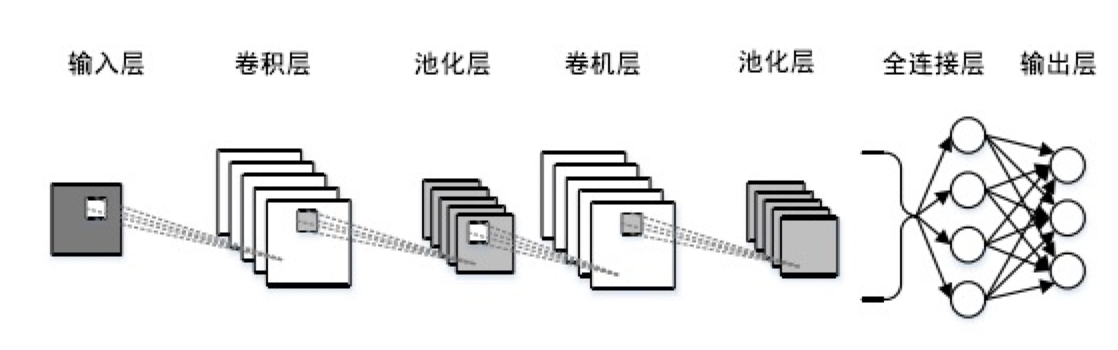
\includegraphics[scale=0.6]{fig2/C5/CNN结构}%联邦学习的系统架构
	\caption{卷积神经网络结构图}
  	\label{fig:卷积神经网络结构图} 
\end{figure}

CNN 网络中的损失函数为 nn.CrossEntropyLoss。该函数是将 nn.LogSoftmax 和nn.NLLLoss 结合起来使用,使用 Softmax 函数和交叉熵损失函数,评估分类任务中的损失,同时可以更加方便地计算反向传播算法。在选择梯度上传的全连接层与传输协议中, 部分超参数选择如下: 选择参数比例 $\theta_{u}=0.01$, 全局参数 $\theta_{d}$ 下载比例为 1 。为了允许在学习中更多的随机性, 将学习率设置为 $\alpha=1 \times 10^{-2}$, 学习速率衰减值为 $1 \times 10^{-7}$ 。参与者迭代过程使用表$\mathrm{CNN}$ 网络训练本地数据集,攻击者使用基于 CNN 网络的 DCGAN算法与成员推理攻击的白盒算法。实验在这样的参数设置下搭建一个包含 29 个正常参与者和 1 个攻击者的 分布式联邦学习系统, 30 个参与者(包含攻击者)都与中央参数服务器进行连接。

我们将与直接增加噪声的情况以及不加噪声的情况进行对比。实验中使用20000 条数据作为训练数据集,每一个客户端拥有 10 个样本的数据,剩下的样本则作为测试数据集,每种情况分别重复做 5 次并取平均值。Adult 实验参数为T = 200,步长 α = 1e − 4 ,衰减系数 γ = 0.99。

\section{自适应扰动方案的实验评估}
对于自适应扰动框架的实验,评估指标主要有隐私预算参数ε,模型预测准确率。梯度自适应加噪的方法对于模型准确度的影响比传统的梯度固定加噪方法更小,在相同的隐私预算约束下,模型准确性有3$\%$左右的提升。首先,对于MNIST数据集,在无差分隐私机制的原始模型上进行训练得到基准测试准确率约为 97$\%$,证明模型结果对于 MNIST 数据集是有效的。 其次,我们分别使用梯度固定加躁方法和梯度自适应加躁方法进行实验,实验结果如下。

(1)使用梯度固定加噪方法:使用所有$D_{p u b}$计算所得的平均梯度0.001作为固定的梯度裁剪阈值进行梯度裁剪,每轮噪声添加的训练批次大小 L 为 600 个样本,因此每个样本的采样率为$\mathrm{q}=\frac{L}{N}=\frac{600}{60000}=0.01$,
噪声量采用中等噪声σ = 5,隐私参数为$\delta=10^{-5}$。如图\ref{fig:梯度固定加噪方法下模型准确率随隐私预算变化情况}所示,隐私预算参数ε为研究变量。随着隐私预算参数越大,差分隐私提供的隐私保护强度越小,噪声量越少,模型的准确率越高。
\begin{figure}[!hbt]
\centering
  	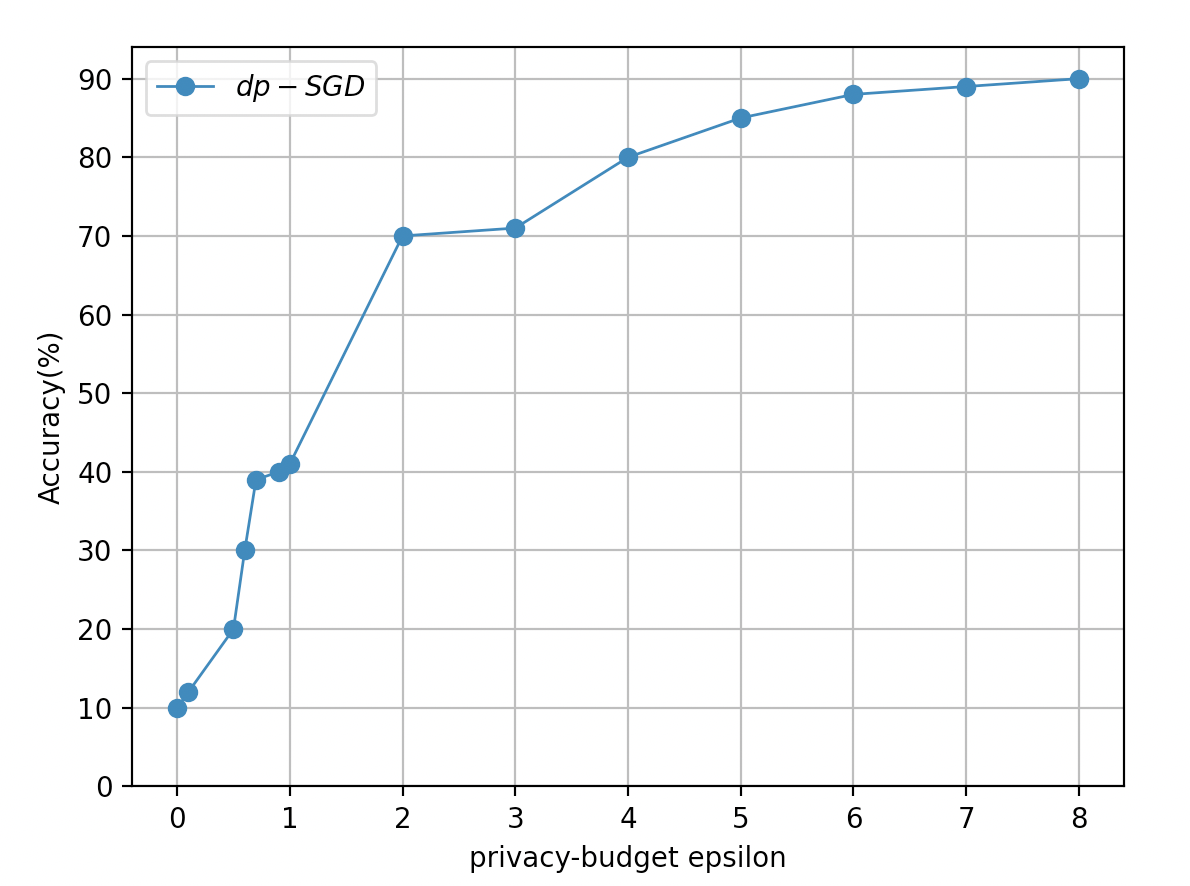
\includegraphics[scale=0.4]{fig2/C5/梯度固定}%联邦学习的系统架构
	\caption{梯度固定加噪方法下模型准确率随隐私预算变化情况}
  	\label{fig:梯度固定加噪方法下模型准确率随隐私预算变化情况} 
\end{figure}

在不同的隐私预算下,随着训练轮数epoc的增加,模型的准确率对比如图\ref{fig:梯度固定加噪方法下模型准确率随隐私预算变化情况 
}所示,ε越大,最终模型预测准确率越高。这时候
隐私预算参数越大,差分隐私提供的隐私保护强度越小,噪声量越少,符合理论原理。当隐私预算$\frac{\epsilon}{c}$≥ 5后,隐私预算参数对于模型准确率影响趋于平稳,综合来看,当$c$≥ 5后,部署了差分隐私机制的模型准确率可达 90$\%$左右,较原始模型存在约 7$\%$的准确率差距。

(2)使用梯度自适应扰动方法:图\ref{fig:梯度自适应扰动方法下模型精度、损失随隐私参数的变化趋势}描绘了目标损失值和准确率随γ变化的趋势,当γ值越小,则越为接近平均分配时的情况。我们可以从图中可以看到,自适应权重在准确率上最高可以提高 6$\%$ 以上,损失值可以降低 0.15 以上。我们可以发现,当 γ 值变小的时候,得到的损失也会相应变大,准确率也会相应变小,整体趋势是随着接近平均的情况效果会下降,这是因为我们根据收敛规律合理分配隐私预算,结果与我们的上文分析所相吻合;另一方面,而当γ过于大的时候,损失很大,准确率很小,整体表现很差,这是因为前期分配的隐私预算过少,导致刚开始的迭代的噪声过大,很难通过后面少量的迭代来弥补。

\begin{figure}[!hbt]
\centering
  	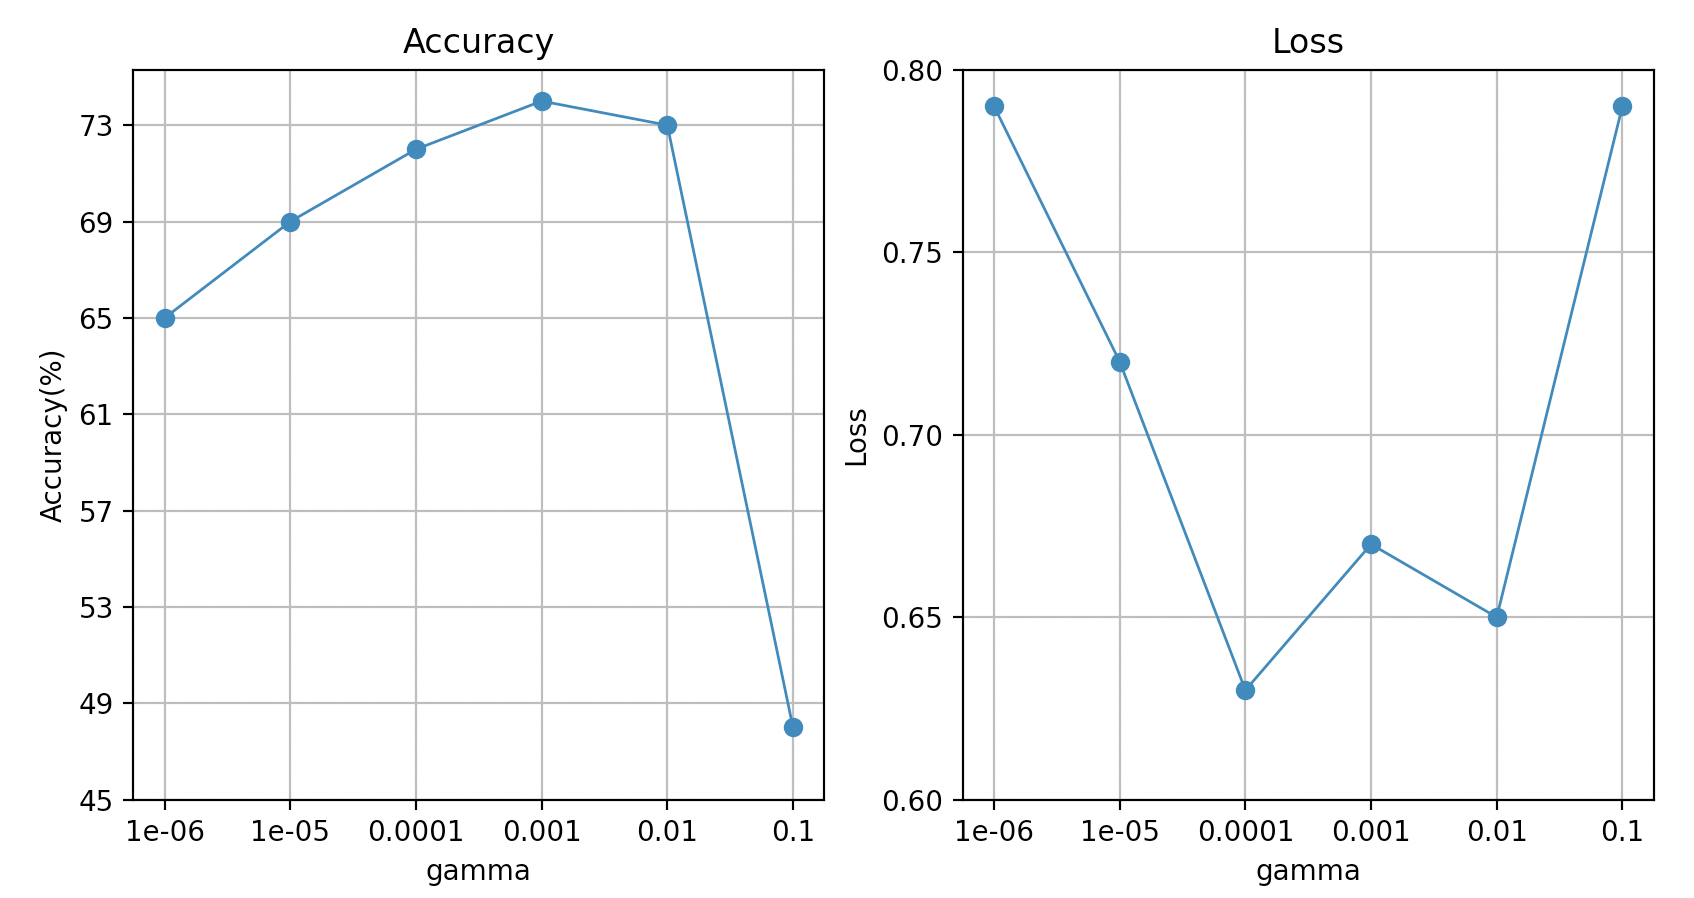
\includegraphics[scale=0.4]{fig2/C5/梯度自适应}%联邦学习的系统架构
	\caption{梯度自适应扰动方法下模型精度、损失随隐私参数的变化趋势}
  	\label{fig:梯度自适应扰动方法下模型精度、损失随隐私参数的变化趋势} 
\end{figure}

接着,我们比较了在不同隐私预算下的自适应干扰模型的准确性,隐私预算分别为($\epsilon$1 = 0.1, $\epsilon$2 = 0.5, $\epsilon$3 = 2.0, $\epsilon$4 = 8.0)。
隐私预算$\epsilon$越小,噪音就越大。我们还为每个隐私预算选择三种不同的参数取值((a): f = 0.15, p = 0.85, (b): f = 0.10, p = 0.90(c): f = 0.05, p = 0.95)。可以肯定的是,设定的(f = 0.15, p = 0.85) 可以保证系统的隐私水平。在实验中,隐私预算ε的值是εc、εl和εc的总和。我们将隐私预算的计算分为以下三个步骤:对于贡献的计算、线性转换中的计算和
和损失函数的计算,即:$\epsilon_{c}=\epsilon_{l}=\epsilon_{f}=\frac{\epsilon}{3}$。

正如图\ref{fig:不同隐私预算的自适应干扰机制在MINIST数据集上的准确率}所示,随着隐私预算ε的增加,我们系统的准确性保持稳定的增长趋势。随着调整因子范围的不断缩小,自适应干扰模型的准确率逐渐降低,但仍保持较高的水平。例如,当隐私预算ε设置为8.0时,在f=0.15和p=0.85的设置下,APFL的准确率高达97.34$\%$,而在f=0.10和p=0.90的设置下,准确率为96.57$\%$,以及在f=0.05和p=0.95的设置下,准确率为96.25$\%$。

\begin{figure}[!hbt]
\centering
  	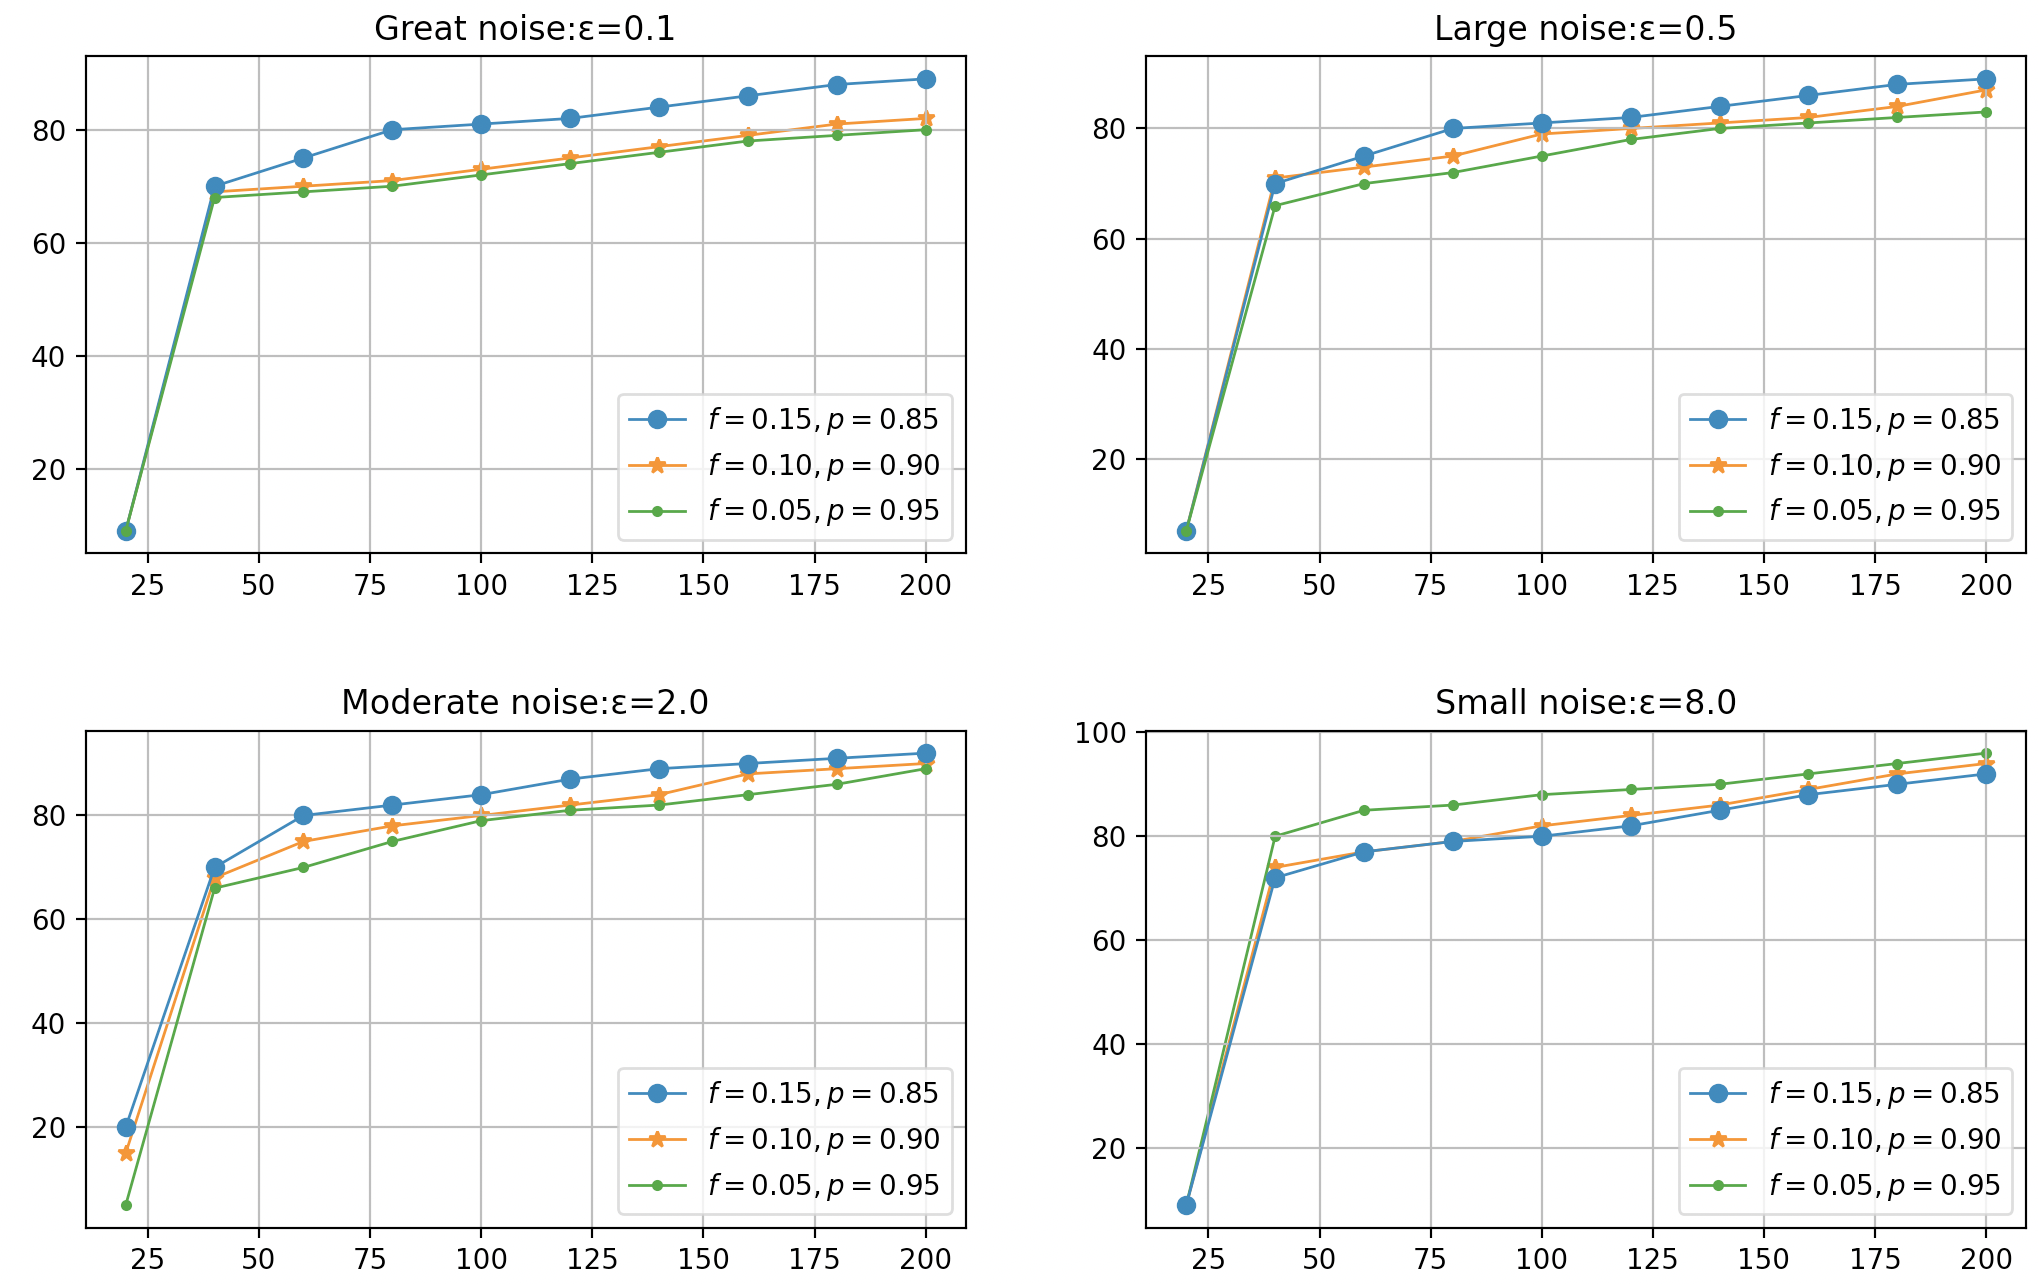
\includegraphics[scale=0.4]{fig2/C5/自适应干扰实验}%联邦学习的系统架构
	\caption{不同隐私预算的自适应干扰模型的准确率}
  	\label{fig:不同隐私预算的自适应干扰机制在MINIST数据集上的准确率} 
\end{figure}

综上,自适应隐私预算分配可以根据一般问题的收敛规律,合理地分配隐私参数,从而提高模型表现,但参数 γ 需要小心选取,过大的 γ 值会导致训练的初始阶段噪声太大,从而影响模型的可用性。

我们还与近年来使用DP机制保护深度学习模型隐私的工作进行了比较,如[1]中的DLPP和[18]中的DSSGD。在图\ref{fig:DP-SGD、DLPP、ACDP在模型准确率和隐私预算上的对比}中,我们可以清楚地得到一个信息,即我们的工作即使在强隐私保证下(ε=0.1)也表现良好。当调整因素设置为f = 0.15和p = 0.85时,模型的准确率在200个历时后达到88.46$\%$。此外,调整因素为f=0.05和p=0.95,自适应干扰模型的准确率为86.79$\%$。然而,在相同的隐私预算下,DP-SGD的准确性仅达到79.63$\%$,DLPP模型的准确性低于65.00$\%$。

\begin{figure}[!hbt]
\centering
  	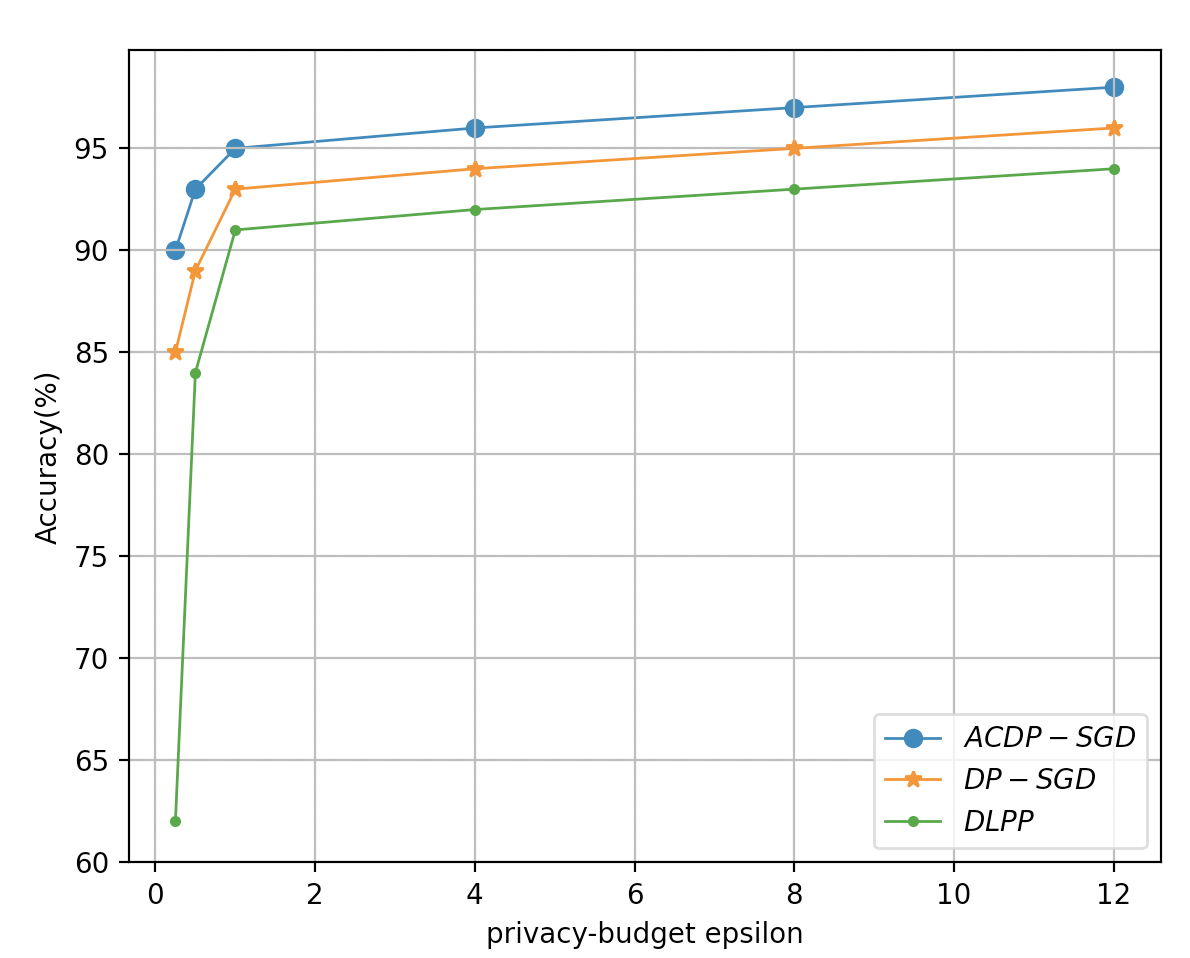
\includegraphics[scale=0.3]{fig2/C5/自适应干扰实验对比}%联邦学习的系统架构
	\caption{DP-SGD、DLPP、ACDP在模型准确率和隐私预算上的对比}
  	\label{fig:DP-SGD、DLPP、ACDP在模型准确率和隐私预算上的对比} 
\end{figure}


\section{安全混洗算法的实验评估}
我们在MNIST、FMNIST和CIFAR上评估所提出的安全聚合框架。为了评估参数:模型迭代次数$f_{r}$,我们首先将客户端的数量固定为500。

如图\ref{fig:安全混洗模型中参与混洗的本地客户端数量对联合模型精度的影响}所示,通过客户端采样机制和梯度的拆分混洗算法,我们的安全混洗模型(下文简称SA-FL)能够以较低的隐私成本实现较高的准确性。在训练中增加客户数量n的同时,SA-FL的表现与无噪声的联合学习一样接近。与MNIST(n=100,ε=1)、FMNIST(n=200,ε=5)相比,CIFAR-10(n=500,ε=10)需要更多的客户端,这表明对于一个具有较大神经网络模型的更复杂的任务,它需要更多的本地数据和更多的客户端以获得对数据扰动的更好表现。

\begin{figure}[!hbt]
\centering
  	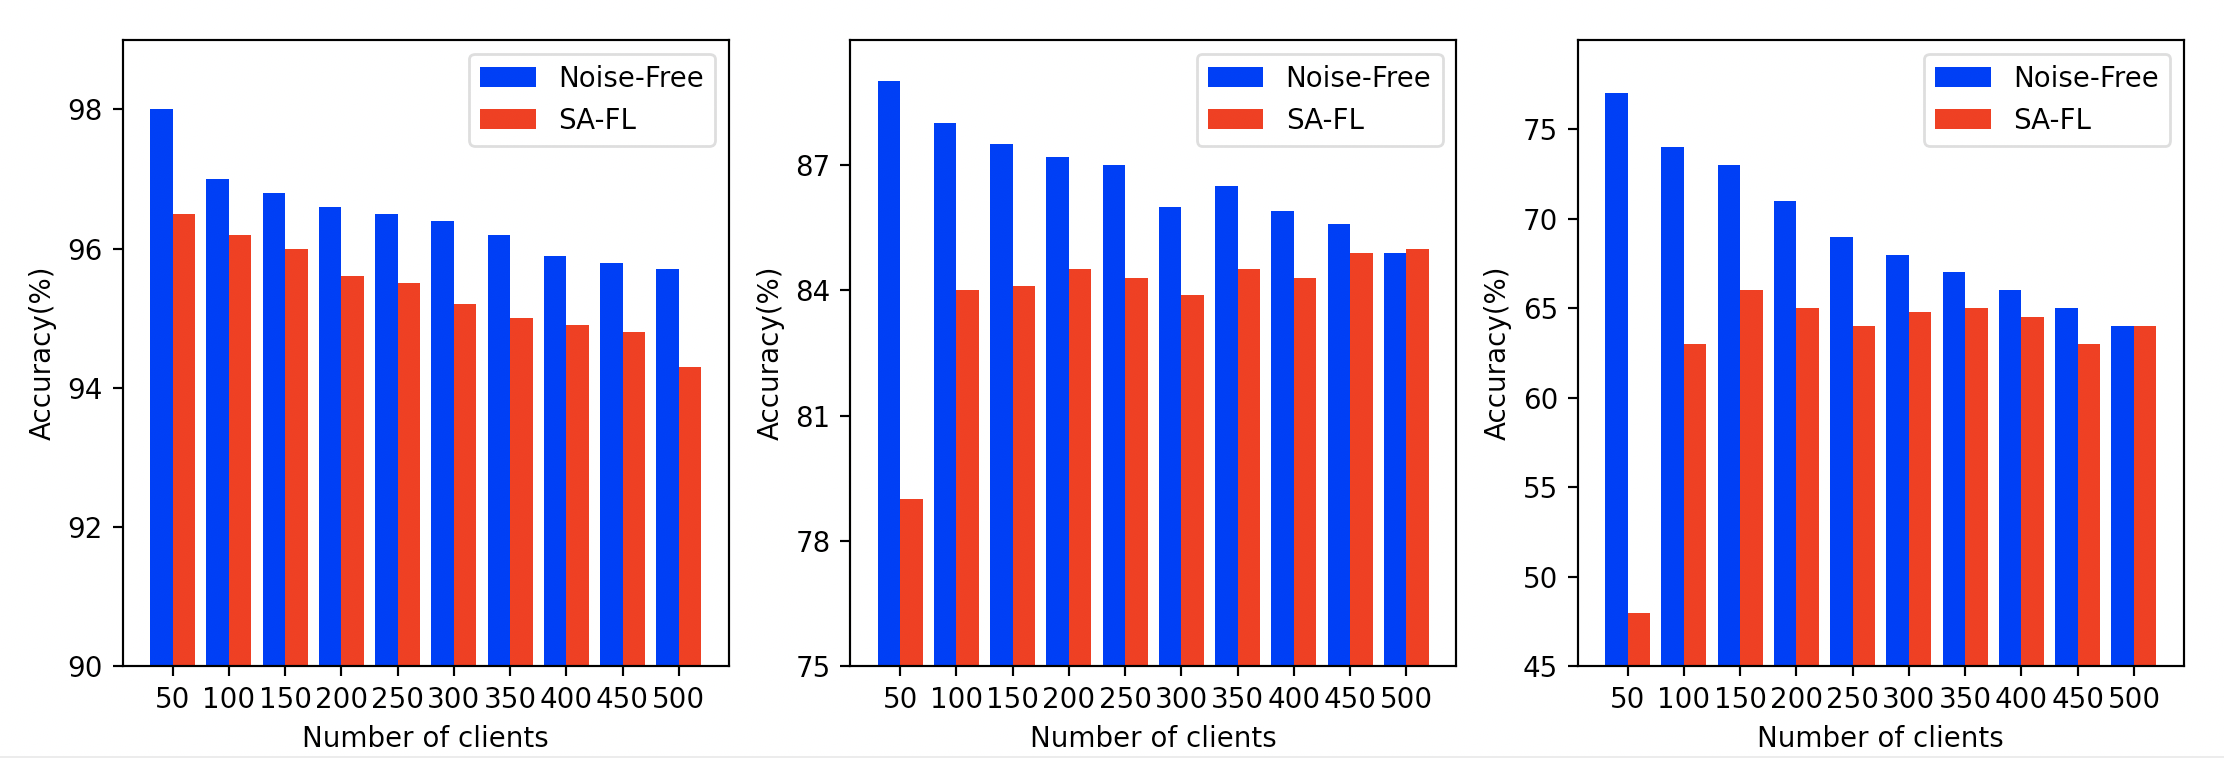
\includegraphics[scale=0.3]{fig2/C5/SA-FL}%联邦学习的系统架构
	\caption{安全混洗模型中参与混洗的本地客户端数量对联合模型精度的影响}
  	\label{fig:安全混洗模型中参与混洗的本地客户端数量对联合模型精度的影响} 
\end{figure}

由图\ref{fig:安全混洗模型中通信轮数和客户端采样比对联合模型精度的影响}可以发现,当$f_{r}$太小的时候,并不影响在MNIST上的表现,但对FASHION-MNIST和CIFAR-10的表现影响很大。当$f_{r}$接近1时,安全聚合框架可以在MNIST、FASHION-MNIST和CIFAR-10上取得与无噪声结果几乎相同的性能。另一个重要的参数是中央参数聚合器和本地客户端之间的通信轮次。不难看出,随着通信次数的增加,我们可以通过所提出的模型在所有数据集上训练出更好的模型。然而,由于数据和任务的复杂性,CIFAR-10需要更多的通信回合以获得更好的模型。

\begin{figure}[!hbt]
\centering
  	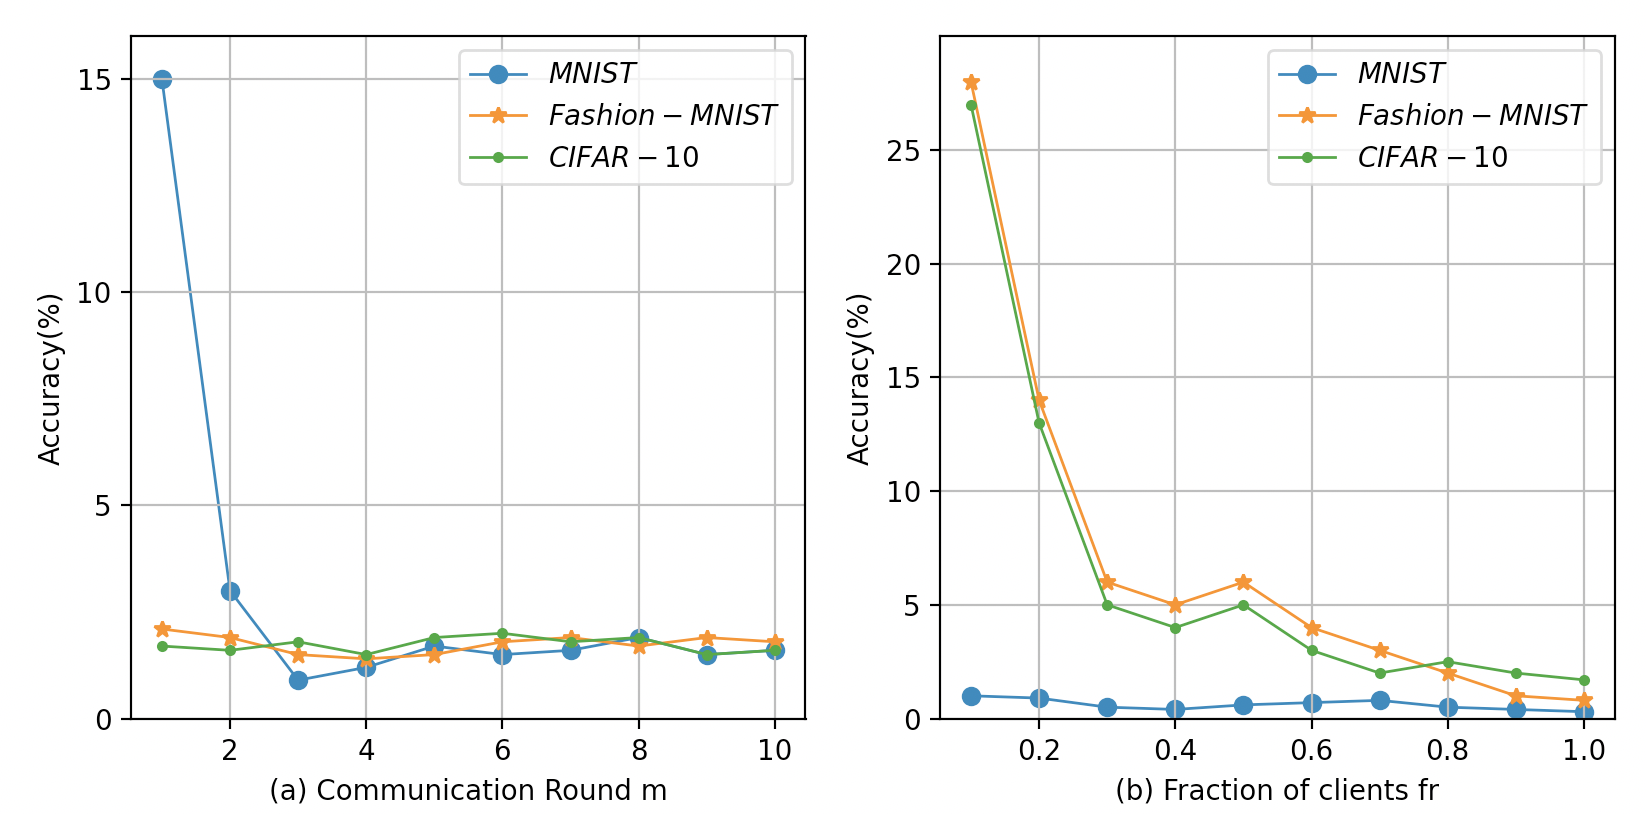
\includegraphics[scale=0.4]{fig2/C5/SA-FL2}%联邦学习的系统架构
	\caption{安全混洗模型中通信轮数和客户端采样比对联合模型精度的影响}
  	\label{fig:安全混洗模型中通信轮数和客户端采样比对联合模型精度的影响} 
\end{figure}

\begin{figure}[!hbt]
\centering
  	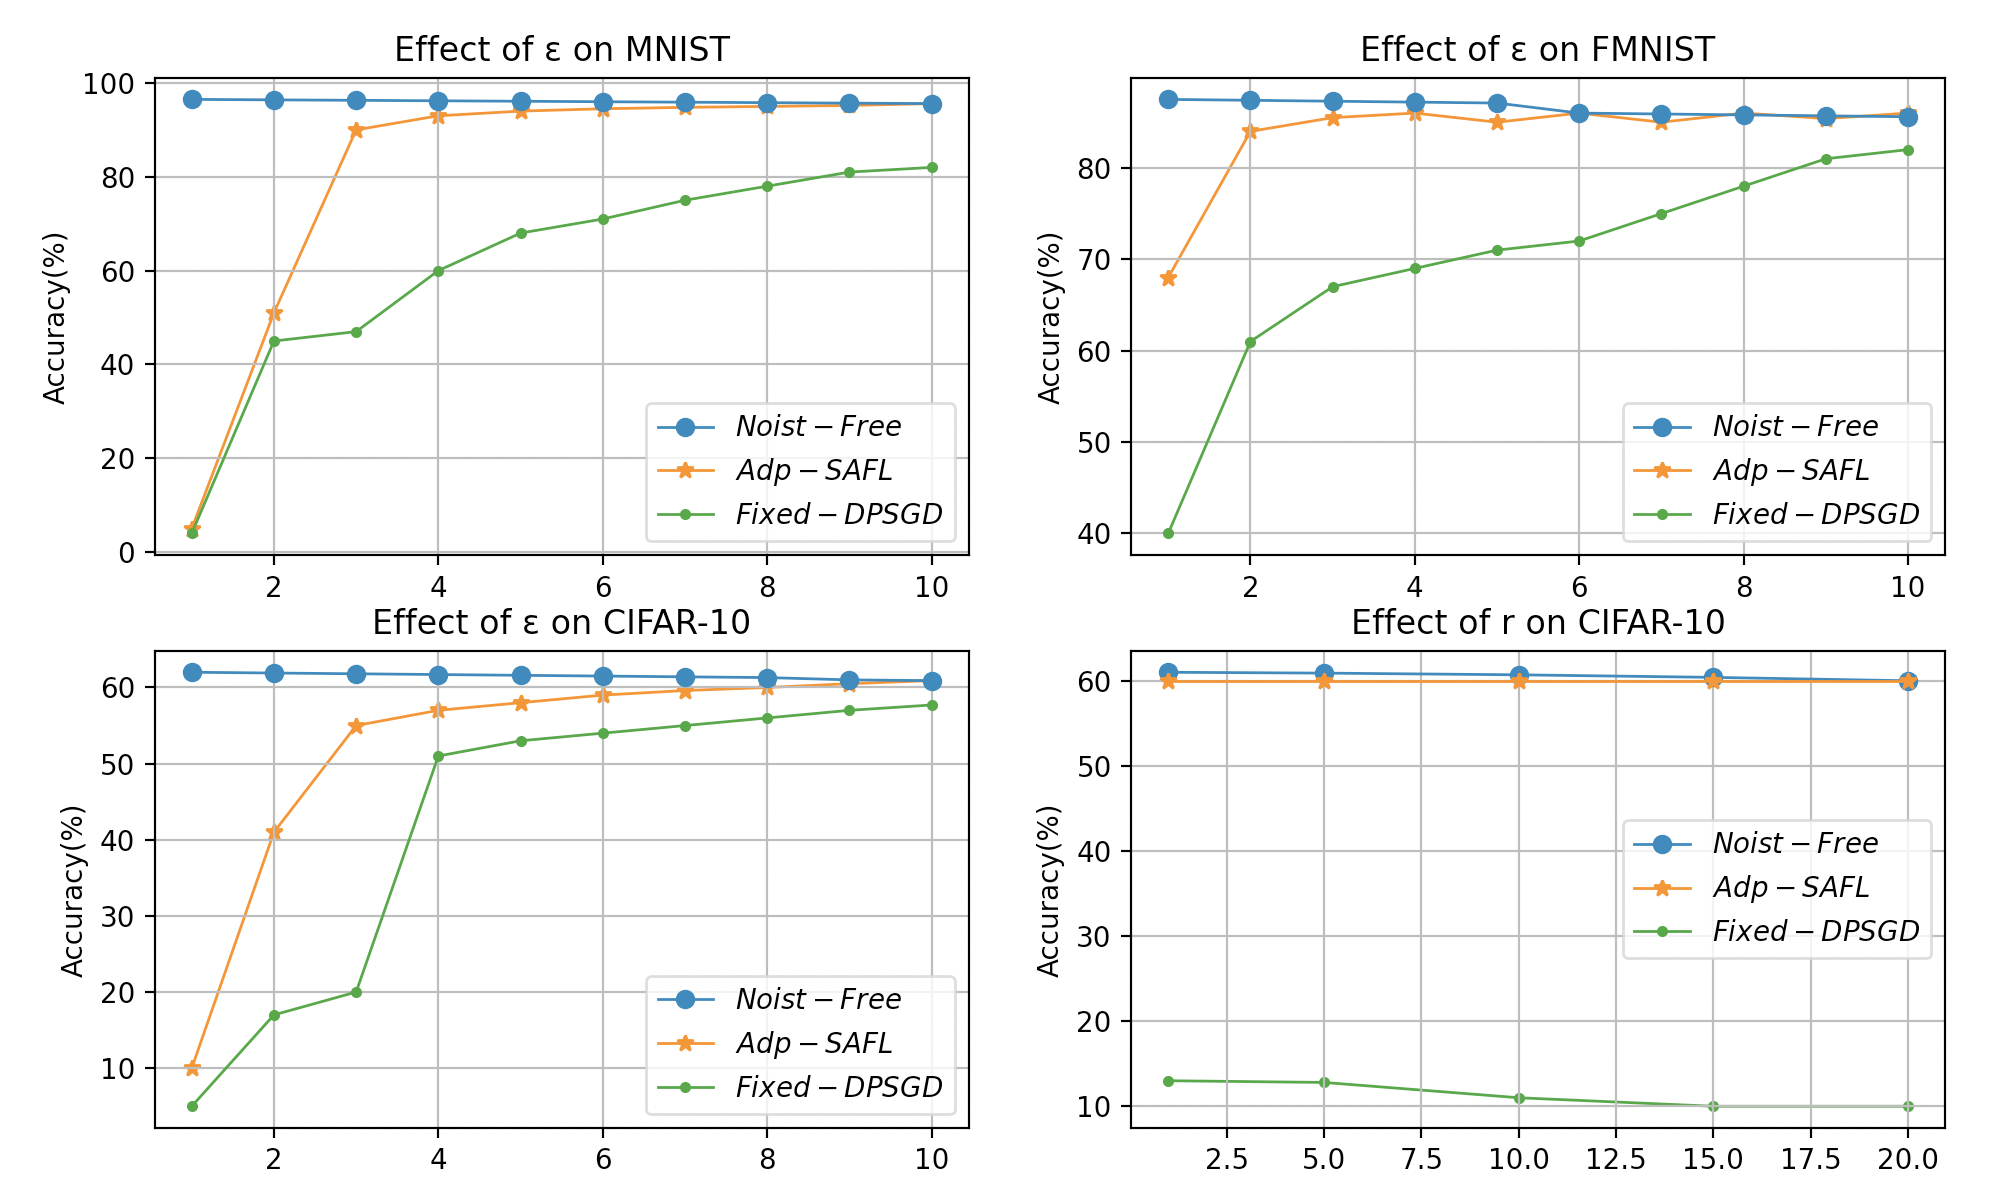
\includegraphics[scale=0.38]{fig2/C5/SA-FL对比实验}%联邦学习的系统架构
	\caption{训练参数对模型精度的影响}
  	\label{fig:[a-c]: 隐私预算对模型准确率的影响; [d]: 参数r对模型准确率的影响} 
\end{figure}

如图\ref{fig:[a-c]: 隐私预算对模型准确率的影响; [d]: 参数r对模型准确率的影响}(a-c)中,SA-FL在ε=1和n=100的情况下可以达到96.24$\%$的准确率,在ε=4,n=200的情况下可以达到86.26$\%$的准确率,在ε=10,n=500的情况下,在MNIST,FMNIST和CIFAR-10上可以达到61.4$\%$的准确率。我们的结果与之前的其他工作相比非常有竞争力。[Geyer等人,2017]首次将差分隐私应用于联邦学习,虽然他们使用了100个客户端,但在MNIST上,他们只能在(ε,m)=(8,11),(8,54)和(8,412)的情况下达到78$\%$,92$\%$和96$\%$的准确率,保证了差异化的隐私,其中(ε,m)代表隐私预算和通信回合。[Bhowmick等人,2018]首次在联合学习中利用本地差分隐私。由于其机制的高变异性,它需要超过200轮的通信,并花费更多的隐私预算,即MNIST(ε=500)和CIFAR-10(ε=5000)。最近的工作[Truex等人,2020]将浓缩的局部差分隐私(α-CLDP)应用到联邦学习中,在FMNIST数据集上获得了86.93$\%$的准确性。然而,α-CLDP通过要求相对较大的隐私预算ε = α-2c-10ρ(例如,α = 1,c = 1,ρ = 10)来实现该性能,这导致了较弱的隐私保证。与以往的工作相比,我们的方法在客户端和云端之间需要更少的通信回合(例如,MNIST为10,FMNIST和CIFAR-10为15),这使得整个解决方案在实际场景中更加实用。总的来说,SA-FL在有效性、效率和维护成本方面都比之前的作品取得了更好的表现。


\section{结果分析}
为了验证自适应扰动算法对于模型训练的精度也能维持在较优的水平,我们进行了对比实验,使用自适应扰动算法和不使用这种方法在不同的隐私参数$\epsilon$下的对比实验。由本章第三节对于自适应差分隐私方案的实验评估,我们可以看到自适应
扰动算法基本上占有绝对的优势,尤其是在损失函数值,在隐私参数$\epsilon$=0.1时,我们的方法不到1,而传统的平均算法却在100左右。这么大的差距的原因在于,自适应扰动算法的权重分配使得聚合时个体信噪比不变,但整体的聚合结果的信噪比却提高了很多,因此当隐私参数$\epsilon$很小,即噪声量很大的时候,表现越好。而当$\epsilon$越大时,注入的噪声也就越小,自适应加躁方法的效果就没有噪声大的时候明显.

系统的额外开销主要来自服务器端的预训练过程,以及用户端在开始训练前对贡献的计算和扰动。我们使用20个历时来训练云服务器的初始化网络,这平均需要68.22秒。在独立和异步的训练过程之前,用户需要用层间依赖传播算法计算权重。这个过程只需要训练正向传播过程,而不需要计算反向传播过程中的梯度和损失惩罚。其平均时间为4.35毫秒。
为了减轻隐私威胁,我们的解决方案是向权重、线性变换函数中的原始数据和损失函数的系数注入拉普拉斯噪声。向权重注入噪声的步骤可以与计算贡献同步进行,这需要额外的2.67毫秒时间。向线性变换中的原始数据和损失函数的系数注入自适应噪声的操作可以在训练前完成,每一个历时的计算都与扰动的权重相似。因此,在模型效率方面的提升是非常突出的。

从隐私成本和模型精度的总体上看,混洗差分隐私方法在各统计问题的结果可用性上都有着相比本地化差分隐私方法明显更优的结果。但从通信代价和计算代价的角度分析,安全混洗算法中混洗器的引入,一方面使得用户数据与用户所使用的编码器之间的关联性消失,使得分析器端的计算代价增大;另一方面促使研究者们使用富含信息更多的多消息模式对数据编码,造成了分析器端的通信代价增大。如何兼顾数据的隐私性、可用性、算法的计算代价和通信代价是后续基于SA-FL框架构建的隐私保护方法需加以考量的部分。从各混洗差分隐私算法评估的结果看,随着的$\frac{\epsilon}{c}$
增大,各方法的数据可用性均会得到提高;而随着用户数据 n 的增加,基于本地化差分隐私方法设计的混洗差分隐私方法在计算误差上会有轻微的增加,其他大多数混洗差分隐私方法在计算误差上没有明显变化,甚至部分方法有着轻微的降低。总体上,基于多消息模式设计的混洗与用户数据相关的信息,有着相对较高的数据可用性,与前文的理论分析相一致。


\section{本章小结}
在本章中,我们选取了三个基准数据集对本文提出的自适应本地差分隐私和安全混洗框架进行了一系列的实验来测试其可行性,并且在联邦学习系统上也进行实验和研究。实验结果表明,我们的自适应本地差分隐私可以有效降低隐私预算,并且维持模型精度。安全混洗框架能通过客户端采样算法和梯度的拆分混洗算法,降低隐私保护预算,提高数据的可用性。

